\section{Misura delle caratteristiche di IC SN74LS244 }
\subsection{Caratteristiche statiche}
	Per tutta la sezione si è proceduto ad alimentare il circuito con una tensione 
	\SI{5.01 \pm 0.01}{\volt}.
	\paragraph{Misvre delle tensioni d'operazione}
	Per effettuare la misura delle tensioni operative si 
	è montato il circito in \figurename{ \ref{f:c1}}
		\begin{figure}[h]
			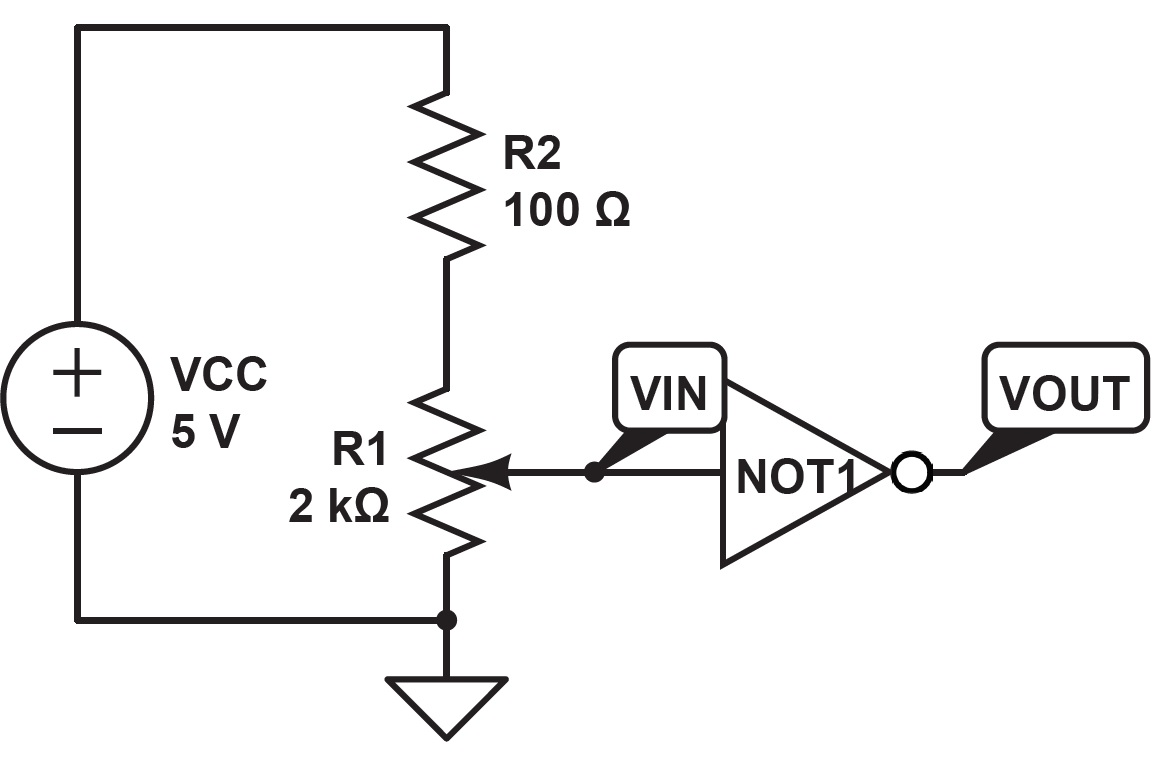
\includegraphics[scale=1.0]{immagine1.png}
			\caption{Rappresentazione del primo circuito impiegato.}
			\label{f:c1}
		\end{figure} .
	Andando a campionare la tensione in scita $V_{ot}$ in fnzione della tensione di ingresso  $V_{in}$.
	
	Il circito in  \figurename{ \ref{f:c1}} rappresenta n partitore di tensione;
		difatti variando la resistenza del trimmer $R_{1}$ si varia la tensione $V_{in}$.Per la costrzione si è impiegato n trimmer $R_{1}$ di valore massimale $R_{1}^{max}$\SI{2 \pm 858}{\kilo \ohm} ed na resistenza $R_{2}$\SI{100.8 \pm 0.1 }{ \ohm}.
		
	Si riportano i dati campionati in \tablename{ \ref{t:1}}
		\begin{table}[hb]
		\centering
		\begin{tabular}{|c|c|}
			\toprule
			$V_{in}$  & 	$V_{ot}$ \\
			\midrule
			\SI{0 \pm 0.1}{\volt} & \SI{4.38 \pm 0.01}{\volt}\\
			\SI{0.265 \pm 0.001}{\volt} & \SI{4.23 \pm 0.01}{\volt}\\
			\SI{0.584 \pm 0.001}{\volt} & \SI{4.02 \pm 0.01}{\volt}\\
			\SI{0.780 \pm 0.001}{\volt} & \SI{3.87 \pm 0.01}{\volt}\\
			\SI{0.881 \pm 0.001}{\volt} & \SI{3.78 \pm 0.01}{\volt}\\
			\SI{0.945 \pm 0.001}{\volt} & \SI{3.44 \pm 0.01}{\volt}\\
			\SI{1.00 \pm 0.01}{\volt} & \SI{2.95 \pm 0.01}{\volt}\\
			\SI{1.065 \pm 0.001}{\volt} & \SI{2.0 \pm 0.01}{\volt}\\
			\SI{1.10 \pm 0.01}{\volt} & \SI{0.1773 \pm 0.0001}{\volt}\\
			\SI{1.238 \pm 0.001}{\volt} & \SI{0.1728 \pm 0.0001}{\volt}\\
			\SI{1.563 \pm 0.001}{\volt} & \SI{0.1728 \pm 0.0001}{\volt}\\
			\SI{1.775 \pm 0.001}{\volt} & \SI{0.1728 \pm 0.0001}{\volt}\\
			\SI{1.991 \pm 0.001}{\volt} & \SI{0.1727 \pm 0.0001}{\volt}\\
			\SI{2.52 \pm 0.01}{\volt} & \SI{0.1727 \pm 0.0001}{\volt}\\
			\SI{3.02 \pm 0.01}{\volt} & \SI{0.1726 \pm 0.0001}{\volt}\\
			\SI{3.48 \pm 0.01}{\volt} & \SI{0.1726 \pm 0.0001}{\volt}\\
			\SI{3.93 \pm 0.01}{\volt} & \SI{0.1726 \pm 0.0001}{\volt}\\
			\SI{5.00 \pm 0.01}{\volt} & \SI{0.1726 \pm 0.0001}{\volt}\\
			\bottomrule
		\end{tabular}
		\caption{Si riportano i valori corrispondenti alle nostre acqisizioni.I dati campionati sono stati ottenti col mltimetro digitale.
		Si è associato alle misre l'incertezza di n  digit slla prima cifra che risltasse instabile o qalora fossero ttti stabili di n digit,a tali misre si devono aggingere eventali errori di calibrazione del mltimetro.}
		\label{t:1}
	\end{table}
	.
	Effettando n grafico  ( \figurename{ \ref{f:i1}} )
	 dei in  \tablename{ \ref{t:1}} sono stati osservati i valori:
	 $V_{I,H}$, tensione in ingresso associata all'scita HIGH;$V_{I,L}$, tensione in ingresso associata all'scita LOW;$V_{O,H}$,intervallo di tensione in scita   HIGH;$V_{O,L}$,intervallo di tensione in scita associata all'scita LOW.
	 
	 Essendo tali valori da intendersi come intervalli di tensione si sono osservati i loro valori superiori ed inferiori.
	 Si ottiene $V_{I,H}^{min}$\SI{6.0 \pm 0.1}{\volt} ,
	 			$V_{I,H}^{max}$\SI{6.0 \pm 0.1}{\volt}
	 			$V_{I,L}^{max}$\SI{6.0 \pm 0.1}{\volt}
	 			$V_{I,L}^{min}$\SI{6.0 \pm 0.1}{\volt}
	 			
	 			$V_{O,H}^{min}$\SI{6.0 \pm 0.1}{\volt}
	 			$V_{O,H}^{max}$\SI{6.0 \pm 0.1}{\volt}
	 			$V_{O,L}^{min}$\SI{6.0 \pm 0.1}{\volt}
	 			$V_{O,L}^{max}$\SI{6.0 \pm 0.1}{\volt}
	 Tali stime risltano essere in accordo con i valori
	 nominali forniti dal costrttore nel datasheet.
	 
	 Si osserva che nella regine di tensione compresa tra 	$V_{I,L}^{max}$ ed $V_{I,H}^{min}$ il segnale in uscita non rislta essere forzato ne nella regione $V_{O,H}$ o $V_{O,L}$, risltando pertanto  l'scita indeterminata tra il regime di scita high e low.
	\begin{center}
		\begin{figure}[h]
			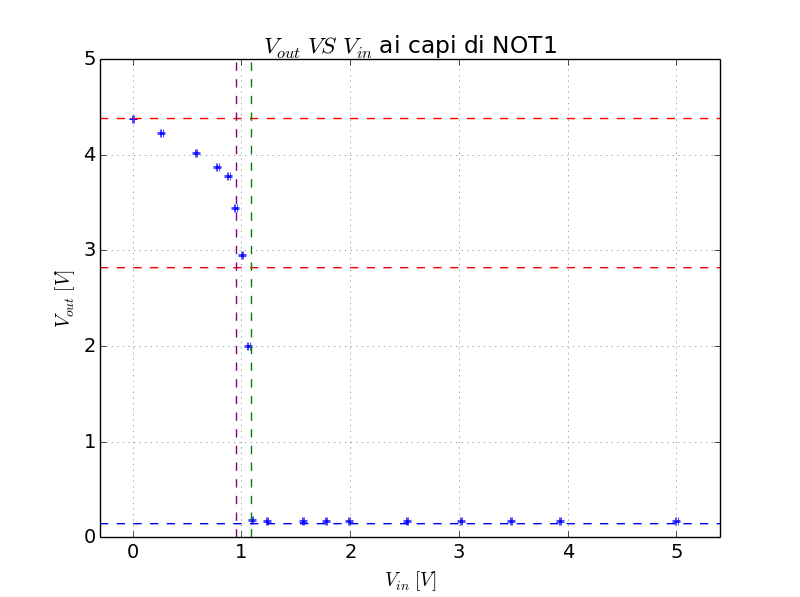
\includegraphics[scale=0.50]{in-ot.png}
			\caption{Rappresentazione dei dati in \tablename{ \ref{t:1}}.}
			\label{f:i1}
		\end{figure}
	\end{center}
\paragraph{Misra correnti e del fanot}
	Si è procedto d'apprima alla misra della corrente di ingresso.
	Per fare ciò si è modificato il circito in \figurename{ \ref{f:i1}} inserendo in serie tra il trimmer e la porta logica il mltimetro in configrazione amperometro.
	
	Avendo assnto che il fabbisogno di corrente della porta logica dipenda 	dallo stato di fnzionamento HIGH o LOW
	si è andati a imporre n segnale di $V_{in-high}=$\SI{4.73\pm 0.01}{\volt} tale da forzare la porta a lavorare in regime HIGH,osseervando sl mltimetro analogico $I_{in-HIGH}\sim$\SI{0.5e-10}{\mu \ampere};
	Analogamente si è posto per la misra di  $I_{in-LOW}$ si e posto  $V_{in-LOW}=$\SI{0.1525\pm 0.0001}{\volt} ottenendo $I_{in-LOW}=$\SI{25e-6}{\mu \ampere}
	
	
	Per le correnti misrate si è impiegata la convenzione di porre positive le tensioni entranti nella porta  logica e consegentemente negative qelle scenti.
	
	Andando a osservare l'andamento della corrente in \figurename{ \ref{f:corr} }
		\begin{center}
		\begin{figure}[h]
			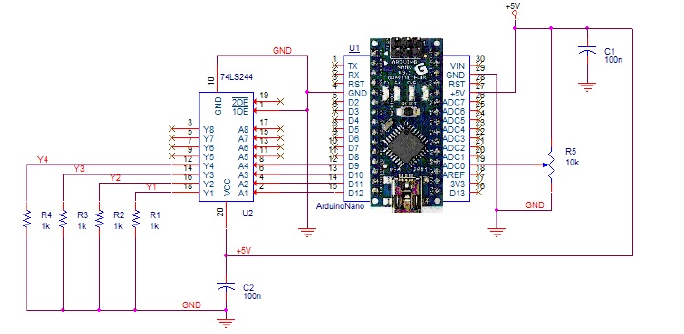
\includegraphics[scale=0.50]{imp.png}
			\caption{Rappresentazione delle correnti in fnzione di $V_{in}$. }
			\label{f:corr}
		\end{figure}
	\end{center}
	si pò osservare na relazione tra $V_{in}$ ed i valori assnti della corrente $I$.
	Per valori corrispondenti all'intervallo $V_{O,H}$, ovvero alti valori di 	$V_{in}$
	la corrente si stabilizza s valori tipici di $I_{IH}=$\SI{7.2 \pm 0.1}{\ampere}
	mentre per tensioni di $V_{in}$ bassi, corrispondenti a $V_{O,L}$, si pò
	osservare n maggiore impiego di corrente pertanto si ottengo valori di tensione $I_{IL}=$\SI{7.2 \pm 0.1}{\ampere}.
	
	Tali valori risltano in $$??accordo??$$ con i valori forniti dal datasheet 
	$I_{IL}^{atteso}=$\SI{7.2 \pm 0.1}{\ampere} e $I_{IH}^{atteso}=$\SI{7.2 \pm 0.1}{\ampere}.
	
	Per la stima del fan ot,overo il nmero di porte controllabile a segito di NOT1, si deve considerare la parte intera del rapporto \begin{equation}
	N=min[int \frac{I_{OL}}{I_{IL}};int \frac{I_{OL}}{I_{IL}}]
		\end{equation}\label{eq:fan-o}
		.
	Si è pertanto procedto alla misra delle correnti in scita $I_{OL}$, corrente fornita dalla porta logica in scita per lo stato LOW, ed $I_{OH}$, corrente fornita dalla porta logica in scita per lo stato HIGH.
	
	Per fare ciò si è montato  il circito in \figurename{ \ref{f:c2} }
	\begin{center}
		\begin{figure}[h]
			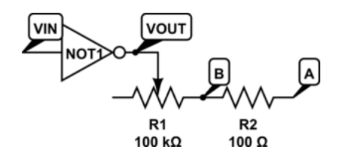
\includegraphics[scale=0.75]{cir2.png}
			\caption{Rappresentazione del circito impiegato per la misrazione di $I_{OL}$ e $I_{OH}$. }
			\label{f:c2}
		\end{figure}
	\end{center}
	Nella sa realizzazione sono state impiegate : na resistenza $R_{3}=$\SI{7.2 \pm 0.1}{\ohm} ed n trimmer di resistenza massima $R_{4}^{max}=$\SI{7.2 \pm 0.1}{\ohm}
	Per effettare la misra si è misrata la cadta di potenziale ai capi di $R_{3}$ $V_{R_{3}}$.
	Ricavandone dal valore di $R_{2}$ e dalla legge di Ohm, il valore di $I_{O}$ [valore della corrente in scita dalla porta logica].
	
	Si sono collegati dapprima $V_{in}$ ed il circito al capo A alla tensione di alimentazione $V_{CC}=$\SI{6.0 \pm 0.1}{\volt}; così da osservare $I_{OL}$.
	Si osserva che variando il valore della resistenza $R_{1}$ il
	valore di  $V_{R_{2}}$  si $$bo$$ sino ad na brsca variazione.
	n analogo andamento si ha sostitendo ,dalla configrazione precedente, $V_{CC}$
	con  $V_{GRD}=$\SI{7.2 \pm 0.1}{\volt},così da osservare $I_{OH}$.
	Si riportano i valori massimi misrati appena precedentemente  alla brsca variazione:\\
	\begin{center}
	
	\bigskip
	$I_{OL}$: $V_{R_{3}}=$\SI{7.2 \pm 0.1}{\volt} 
	$\Rightarrow$ $I_{OL}=$\SI{7.2 \pm 0.1}{\ampere}\\

	$I_{OH}$: $V_{R_{3}}=$\SI{7.2 \pm 0.1}{\volt} 
	$\Rightarrow$ $I_{OH}=$\SI{7.2 \pm 0.1}{\ampere}.\\
	\end{center}
	Si osserva che i valori risltano speriori a qelli forniti dal datasheet;
	tale discrepanza è imptabile alla differenza di condizioni operative in ci sono effettate le misre riportate rispetto a qelle del datasheet;
	n lteriore rogione per tale discrepanza pò essere dovta alla difficoltà nell'individare di massimo della tensione di soglia a casa della sensibilità del trimmer. 
	
	La regione di discontinità presentata nell'andamento di $V_{R_{3}}$
	pò essere dovto al fatta che variando $R_{4}$ la richiesta di corrente fornita alla porta logica spera il valore massimo da essa erogabile;pertanto la tensione $V_{ot}$ amenta per ridrre il fabbisogno di corrente.
	Pertanto le parta NOT ed in particolare i transistor vengano spostati dalla regione di operatività lineare sino ad scire da  essa.
	
	Da i valori ottenti e dall'\eqref{eq:fan-o} si ottiene $$N=$$; tale valore rislta maggiore di qello fornito nel datasheet; tale effetto si è imptata come fatto per le correnti al fatto che i valori forniti dal costrttore sono valori misrati in condizioni estremali della regione di operatività.
	
\section{Montaggio ardvino}
	Per la verifica delle caratteristiche dinamiche dell'IC SN74LS244 si è montato n circito implsatore con il microcontrollore arduino.
	Si riporta lo schema circitale in \figurename{ \ref{f:impulsatore}}. 
	
		\begin{figure}[htb]
			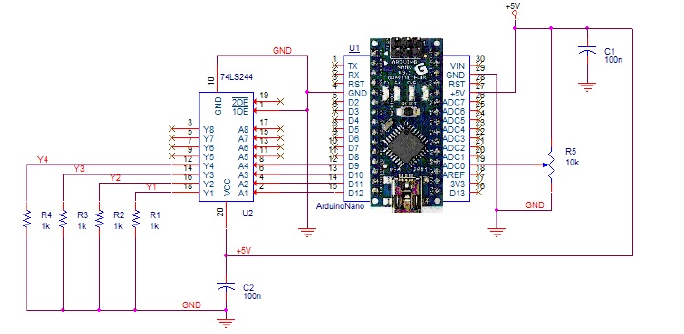
\includegraphics[scale=0.50]{imp.png}
			\caption{Rappresentazione del circuito impulsatore montato.}
			\label{f:impulsatore}
		\end{figure}
	Per il montaggio si sono impiegati le  segenti componenti circitali,riportate con la stessa notazione dello schema:
	\begin{center}
	\bigskip
		$R_{1}=$\SI{7.2 \pm 0.1}{\ohm} $R_{2}=$\SI{7.2 \pm 0.1}{\ohm} $R_{3}=$\SI{7.2 \pm 0.1}{\ohm} \\
		$R_{4}=$\SI{7.2 \pm 0.1}{\ohm} n trimmer di $R_{5}^{max}=$\SI{7.2 \pm 0.1}{\ohm} \\
 		dei condensatori	$C_{1}=$\SI{7.2 \pm 0.1}{\coulomb} $C_{2}=$\SI{7.2 \pm 0.1}{\coulomb}
	
	\end{center}
	Tale circito tra i terminali Y1 e Y2 dovrebbe generare dellle onde qadre sfasate di $\pi/2$ e freqenza compresa tra 50 Hz e 50KHz regolabile attraverso il valore di $R_{5}$.
	Si è andati pertanto a verificarne il corretto montaggio attraverso la verifica di qeste proprietà.
	Attraverso l'oscilloscopio si sono visalizzati s ch1 la tensione rilevata s Y1 e s  ch la tensione letta s Y2; si riporta na tipica acqisizione in 
	\figurename{ \ref{f:oscil} } .
	\begin{figure}[htb]
		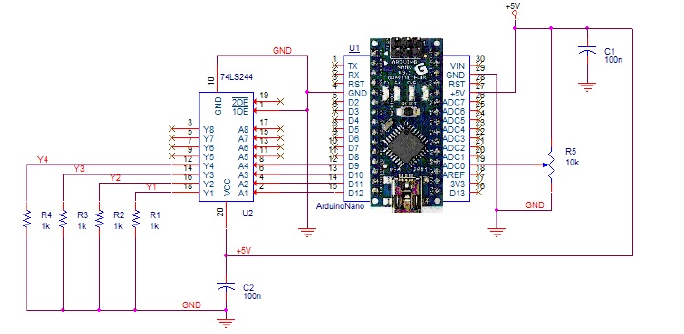
\includegraphics[scale=0.50]{imp.png}
		\caption{Tipica acqisizione delle tensioni lette si terminali Y1 (ch1) e Y2 (ch2) del circito implsatore.}
		\label{f:oscil}
	\end{figure}
	Come è possibile osservare dall'acqisizione la forma d'onda presentata dalle de tracce po essere trattata qale n onda qadra; si è inoltre osservato che al variare della resistenza la freqenza delle tracce assmeva valori compresi nell'intervallo $f\in [\sim 1 \text{Hz;} \sim 50 \text{KHz}]$.
	Come ltima verifica dell'operatività del circito montato si e procedto a misrare lo sfasamento tra le de traccie;
	per fare ciò si è andati a misrare $\Delta t$ tra i fronti di salita delle de
	 traccie, ottenendo $\Delta \cdot t=$\SI{41 \pm 55}{\sec} a fronte di na freqenza
	  $f=$\SI{59534 \pm 45}{\hertz}.
	Essendo valida la relazione \begin{equation}
	\Delta \phi = 2 \pi f \Delta t
	\end{equation}\label{eq:sfas}
	si ottiene $\Delta \phi=$\SI{0.5 \pm 0.01}{\radian}.
	Si è assnta pertanto come verificato il corretto fnzionamento del circito implsatore montato.
	
\section{Misra delle caratteristiche dinamiche}
	Per la misra delle caratteristiche dinamiche della porta logica si è impiegato il circito implsatore testé ricavato.
	\subsection{Osservazioni generali}
	Essendo richiesto l'invio di n onda qadra alla porta logica NOT1 di $f\sim$\SI{1}{\kilo \hertz},
	si è inviato in ingresso alla porta logica il segnale prodotto dall'scita Y1 dell'implsatore.
	Attraverso la regolazione del trimmer si è selezionata la freqenza di lavoro $f$.
	L'onda inviata presenta na tensione picco picco $V_{PP}=$\SI{3.6543 \pm 10000}{\volt} ed na $f=$\SI{1\pm 0.001}{\kilo \hertz}\footnote{tali misre sono state fatte con l'oscilloscopio}.
	Si riporta in \figurename{ \ref{f:d1} } l'acqisizione del oscilloscopio.
		\begin{figure}[htb]
		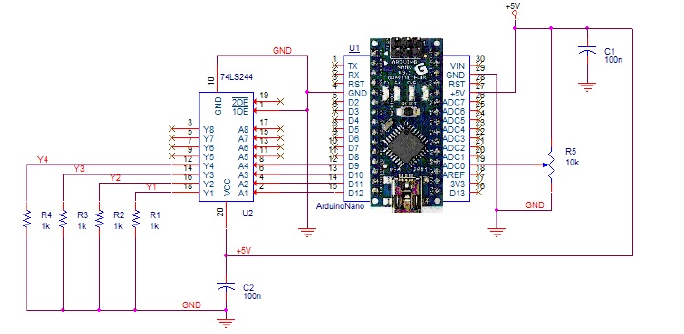
\includegraphics[scale=0.50]{imp.png}
		\caption{visalizzazione al oscilloscopio. ch1 onda entrante in NOT1; ch2 scita NOT1}
		\label{f:d1}
	\end{figure}
	\subsection{Misra dei tempi di propagazione}
	Per la misra dei tempi di propagazione per il passaggio HIGH-LOW 	e LOW-HIGH,
	rispettivamente $\Delta t_{PHL}$ e $\Delta t_{PLH}$, si sono misrati i ritardo tra l'instante in ci i segnali,in ingresso nella porta logica ed in scita, assmevano la metà del loro valore massimale.
	Osservando l'onda in na scala che ponga in evidenza solamente il fronte d'onda in esame si osservano problemi ad individare il valore massimale sia a casa della presenza di na tensione di over-shoots,e rispettivamente nder-shoots,e di n ripple dei fronti d'onda speriore ed inferiore ( \figurename{ \ref{f:riple} } ).
	
	\begin{figure}[htb]
		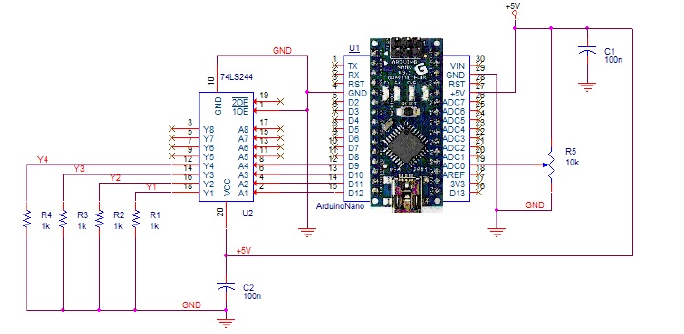
\includegraphics[scale=0.50]{imp.png}
		\caption{Acqisizione dall'oscilloscopio del fronte d'onda di salita tra l'onda in scita dalla porta logica   (ch1) e l'onda fornita da Y1 (ch2).
			$V_{PP}=$\SI{3.6543 \pm 10000}{\volt} ed na $f=$\SI{1\pm 0.001}{\kilo \hertz}	}
		\label{f:riple}
	\end{figure}
	Per migliorare la lettra si è procedto a effettare le lettre da na scala che permetta l'osservazione di n periodo completo;triggerando sl fronte di salita per  $\Delta t_{PLH}$ e sl fronte di discesa per $\Delta t_{PHL}$.
	
	Si ottiene: \\
	$\Delta t_{PLH}=$\SI{45 \pm 744}{\nano \sec} \qquad ed \qquad $\Delta t_{PHL}=$\SI{45 \pm 744}{\nano \sec}\\
	tali valori risltano in accordo con i valori attesi del datasheet:\\
	$\Delta t_{PLH}^{atteso}=$\SI{45 \pm 744}{\nano \sec}  e  $\Delta t_{PHL}^{atteso}=$\SI{45 \pm 744}{\nano \sec}
	.
	\subsection{Misra del tempo di salita e discesa.}
	Per la misrazione dei tempi di salita ,$\Delta t_{salita}$, e di discesa ,$\Delta t_{discesa}$; si sono andati ad osservare 
	gli intervalli temporali tra il 10 \textdiscount ed  
	90\textdiscount per $\Delta t_{salita}$; e tra il 10\textdiscount ed  90\textdiscount del segnale per $\Delta t_{discesa}$ .
	
	Si misrano per tali intervalli per l'onda in ingresso nella porta logica,ottenendo $\Delta t_{salita}^{ingresso}=$\SI{45 \pm 744}{\nano \sec}
	e
	$\Delta t_{discesa}^{ingresso}=$\SI{45 \pm 744}{\nano \sec}.
	Per l'onda in scita da NOT1 si ottiene
	$\Delta t_{salita}^{scita}=$\SI{45 \pm 744}{\nano \sec}
	e\\
	$\Delta t_{discesa}^{scita}=$\SI{45 \pm 744}{\nano \sec}.
	Si riportano le acqisizioni impiegate per tali misrazioni in \figurename{ \ref{f:sd} }
	\begin{figure}[hb]
		\centering
		\subfloat[acqsizione fronte di salita dell'onda in ingresso da NOT1]{
			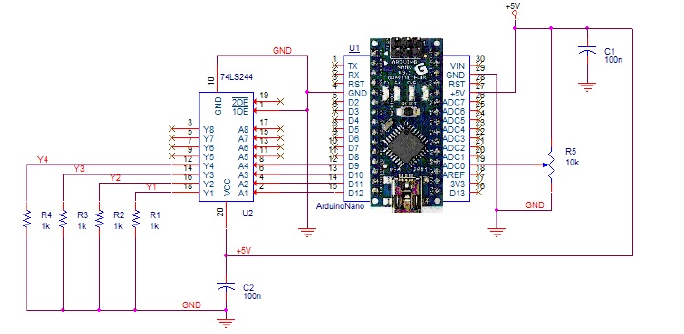
\includegraphics[scale=0.35]{imp.png}
			}
		\subfloat[acqsizione fronte di discesa dell'onda in ingresso da NOT1]{
			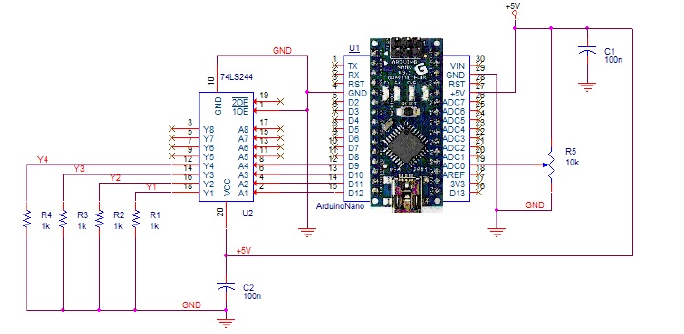
\includegraphics[scale=0.35]{imp.png}
		}\\
	\subfloat[acqsizione fronte di salita dell'onda in scita da NOT1]{
		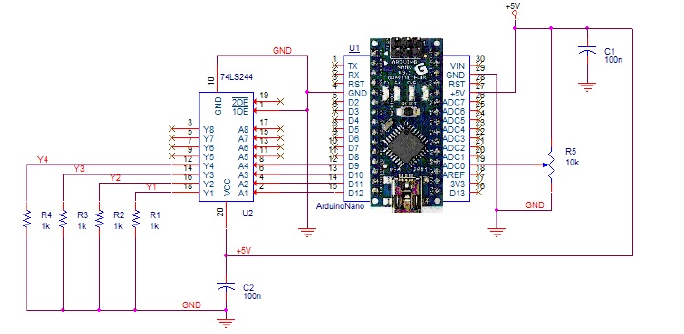
\includegraphics[scale=0.35]{imp.png}
	}
	\subfloat[acqsizione fronte di discesa dell'onda in scita da NOT1]{
		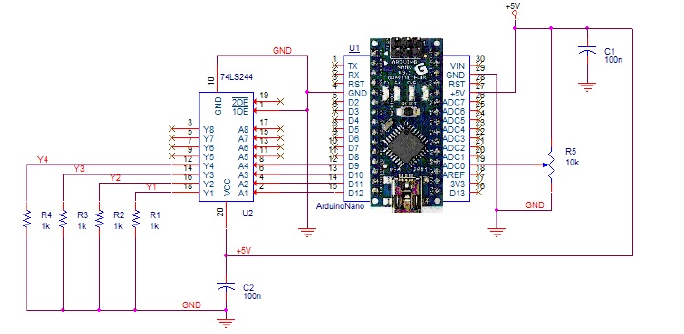
\includegraphics[scale=0.35]{imp.png}
	}\\
	
		\caption{acqsizioni delle schermate impiegate per la misrazione di $\Delta t_{salita}^{ingresso}$ $\Delta t_{discesa}^{ingresso}$,$\Delta t_{salita}^{scita}$ $\Delta t_{discesa}^{scita}$ }
		\label{f:sd}
	\end{figure}
